\chapter{Uma Proposta de Otimização dos Parâmetros do MTSP com Otimizadores Globais}

O modelo proposto consiste em usar um algoritmo de base para calcular as melhores soluções para uma instância do MTSP, enquanto um algoritmo otimizador global procura os melhores conjuntos de parâmetros para o algoritmo base. Algoritmo otimizador global tanto pode ser mono objetivo como pode trabalhar com multiplos objetivos. Neste trabalho, o \textit{Team Ant Colony Optimization} (TACO) é utilizado como algoritmo de base. Além disso, a Otimização de Enxame de Partículas (PSO), a Busca em Cardume de Peixes (FSS) e sua versão multi-objetivo (MOFSS) participam da otimização dos valores dos parâmetros TACO.

\begin{figure}[htb]
    \centering
    \caption{\label{fig:proposal-diag}Modelo de otimização associado a um otimizador global (OG)}
    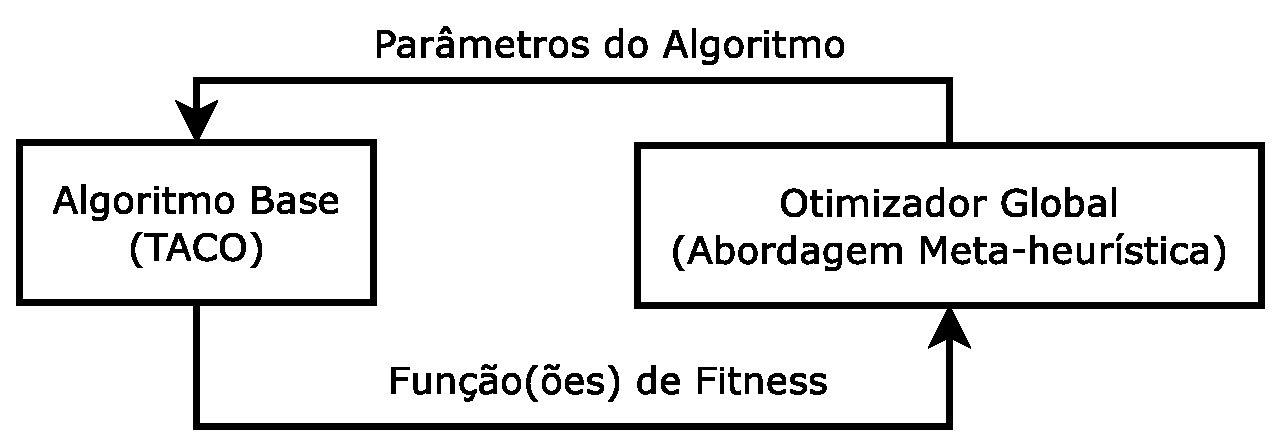
\includegraphics[width=0.75\textwidth]{imagens/proposal-diag.eps}
    \legend{Fonte: o próprio autor.}
\end{figure}

Conforme mostrado na Figura \ref{fig:proposal-diag}, o Otimizador Global (OG) começa a gerar um conjunto de valores para os parâmetros do TACO. Neste caso, os parâmetros otimizados do TACO são $\alpha$, $\beta$, $\xi$ e $\rho$. Então, a TACO constrói um conjunto de melhores soluções baseadas nos parâmetros otimizados. Em seguida, o TACO retorna ao OG o conjunto das melhores soluções, que são avaliadas para o algoritmo meta-heurístico. Conforme as iterações acontecem, o OG mantém um registro do melhor conjunto de parâmetros, que foram encontrados até o momento. A execução termina quando o OG atinge o limite de iterações.

% ---
\section{O Problema: distribuição de medicamentos}
\label{sec-metodologia-problema}
% ---

Uma CAF (Central de Abastecimento Farmacêutico) usualmente executa os pedidos de forma manual, tanto a separação da carga quanto o percurso estabelecido, independente do tempo gasto pelos entregadores. Devido à esta grande variação de tempo necessário no atendimento de pedidos, é difícil estabelecer uma capacidade para cada entregador, no intuito de mitigar os custos individuais dos percursos estabelecidos.

A metodologia deste trabalho consiste na criação de instâncias de MTSP a partir do ambiente real hospitalar e na aplicação de algoritmos baseados no ACO para a construção otimizada de soluções na distribuição de medicamento entre os entregadores.
%COLORIR IMAGEM PARA DESTACAR O PONTO EM VERMELHO
Para este trabalho, foi desenvolvido uma instância MTSP tendo como base um hospital de grande porte, contendo farmácias satélites (FS) e uma CAF. Estas FSs estão distribuídas em diferentes blocos dentro do hospital e em diferente pavimentos. Na Figura \ref{fig:dataset-map} estão destacadas em preto as 16 farmácias em uma simulação para entregas durante o período diurno de um dia típico de trabalho. O ponto em cinza claro está destacado a CAF, local onde os entregadores iniciam e concluem os seus percursos.

\begin{figure}[htb]
    \centering
    \caption{\label{fig:dataset-map}Representação gráfica das farmácias e o CAF num grande hospital} 
    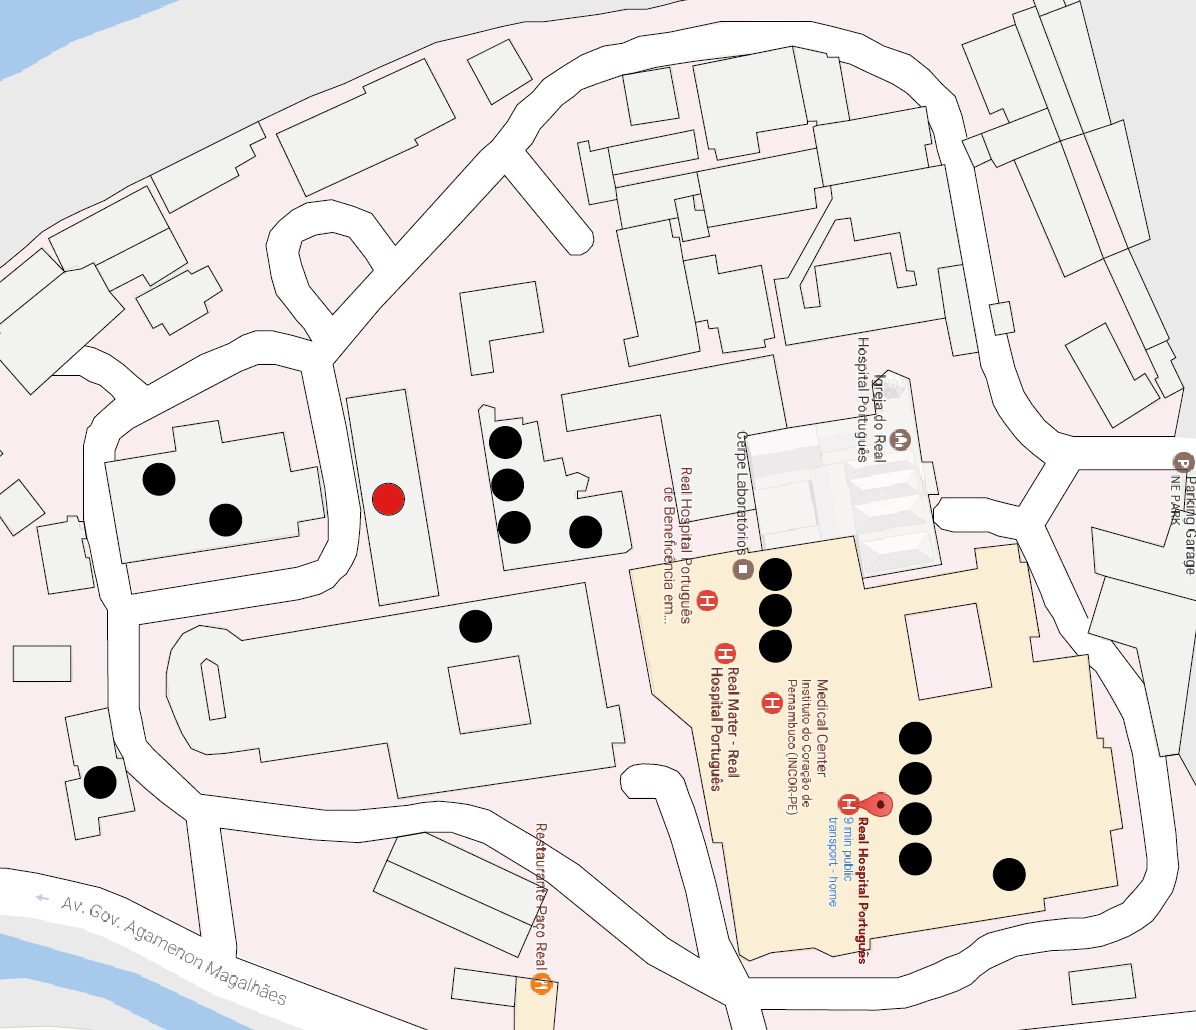
\includegraphics[width=0.75\textwidth]{imagens/dataset-map.png}
    \legend{Fonte: o próprio autor}
\end{figure}

Já na Figura \ref{fig:dataset-graph} mostra o grafo com os vértices representando cada farmácia satélite incluindo o centro de distribuição representado pelo vértice $V_1$, com os respectivos custos em suas arestas, cada mensageiro sai do vértice $V_1$, realiza a rota determinada pelo algoritmo e retorna para o centro de distribuição, $V_1$. Neste grafo há 17 nós (vértices) sendo cada nó $n$ é interligado aos outros $17 - n$ nós. Além disso, para esta abordagem, o problema é considerado como estático, isto é, todos os pedidos são feitos até as 8h da manhã pelas outras farmácias não considerando pedidos feitos depois do tempo limite.

\begin{figure}[htb]
    \centering
    \caption{\label{fig:dataset-graph}Modelo representado em forma de grafo com as suas arestas contendo as distâncias} 
    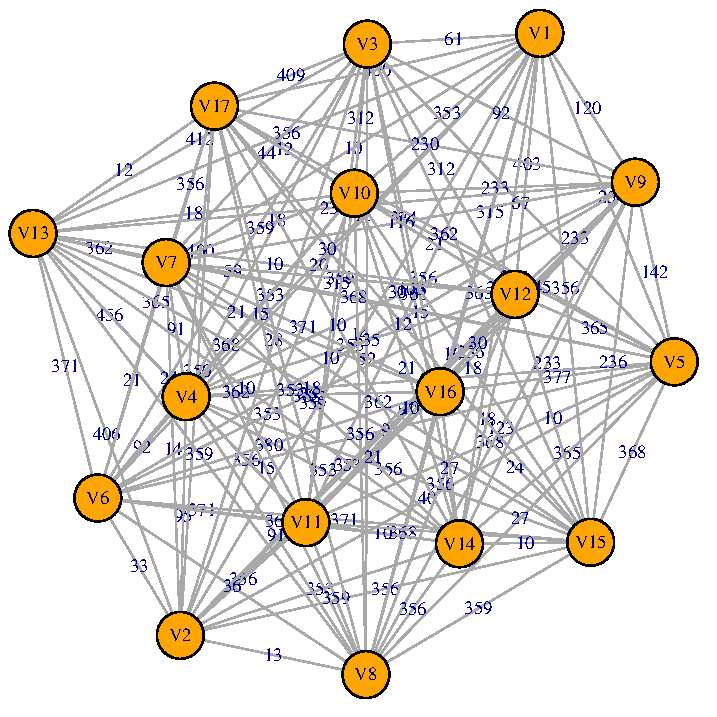
\includegraphics[width=0.75\textwidth]{imagens/dataset-graph.pdf}
    \legend{Fonte: o próprio autor.}
\end{figure}

Uma matriz, chamada matriz de custo, contém os dados de cada farmácia, como número de registro ($id$), latitude, longitude e sua distância. A matriz ajuda a calcular o custo da rota. Da mesma forma, outra matriz, chamada de matriz de dados, contém as ordens de entrega para cada nó no modelo construído. Cada pedido contém registros do remetente e da farmácia, as distâncias iniciais e finais, quando o remetente deixou o CAF e a duração do pedido. A matriz de dados ajuda a simular um dia de pedido no depósito. Além disso, há quatro entregadores para entregar os pedidos às farmácias.

% ---
\section{Parâmetros a serem otimizados}
\label{sec-metodologia-parametros}
% ---

%CORRIGIR NÚMERO DE EQUIPES
Como afirmado anteriormente, um otimizador global, baseado em inteligência de enxame, também é usado para melhorar os resultados do TACO, otimizando seus parâmetros. FSS, MOFSS e PSO são considerados como um otimizador global dos parâmetros TACO. Os valores padrão para o conjunto de parâmetros utilizados são: número de entregadores $M = 4$, número de equipes $N = 10$, probabilidade inicial $q_0 = 0,5$, relevância de feromônio $\alpha = 0,5$, relevância de visibilidade $\beta = 1,0$, persistência de feromônio para atualização local $\xi = 0,1$, persistência de feromônio para atualização global $\rho = 0,1$. Esses valores padrão foram obtidos por um teste de parâmetro. O critério de parada é de 1000 iterações para cada execução independente. Os otimizadores globais otimizam o subconjunto de parâmetros $P = \{\alpha, \beta, \xi, \rho\}$ em um intervalo de $0 \leq P \leq 2$.

% ---
\section{Metodologia Experimental}
\label{sec-metodologia-experimento}
% ---

Os experimentos apresentados nesta seção têm como objetivo mostrar a eficácia da metodologia desenvolvida aplicada ao problema real. No primeiro cenário, os algoritmos são configurados para minimizar o custo total das soluções, sem considerar a distribuição da carga de trabalho entre as equipes, como na descrição geral do MTSP. No segundo cenário, os algoritmos minimizam o custo da maior rota individual das soluções, visando a construção de soluções formadas por rotas com custos iguais entre os entregadores, como no MTSP com balanceamento de carga de trabalho.

% ---
\subsection{Ambiente de Simulação}
\label{subsec-metodologia-experimento}
% ---

Todos os experimentos foram executados em um MacBook Pro (13 polegadas, final de 2011) com CPU Intel Core i5 de 2,4 GHz, 16 GB de RAM (1333 MHz DDR3) e sistema operacional MacOS High Sierra (versão 10.13.4). Usamos o banco de dados apresentado na Seção \ref{sec-metodologia-problema}. Em seguida, realizamos 30 execuções independentes dos algoritmos para cada experimento. O algoritmo TACO foi codificado em Java com base no algoritmo proposto por Valivaara (2007) e está disponível em \url{https://github.com/renanalencar/taco-mofss.git}. O FSS é baseado na versão de Verçosa, Bastos-Filho e Monteiro (2017) \cite{verccosa2017combining}. O PSO de objetivo único foi retirado da estrutura do jMetal (DURILLO; NEBRO, 2011) \cite{durillo2011jmetal}. O MOFSS utilizado é baseado na versão de Bastos-Filho e Guimarães (2015) \cite{bastos2015multi} utilizando o jMetal como framework para visualizações.

O TACO desenvolvido por Valivaara foi utilizado por ter apresentado bons resultados na resolução de problemas do tipo MTSP durante experimentos prévios no desenvolvimento deste trabalho. O algoritmo foi codificado em Java para facilitar a integração com outras ferramentas já disponíveis e algoritmos utilizados como OGs. Já o FSS desenvolvido foi escolhido Verçosa, Bastos-Filho e Monteiro por ter como base a versão FSS Vanilla (disponível em \url{http://www.fbln.pro.br/fss/versions.htm}) e apresentar estruturação das classes compatível com os problemas da Conference on Commerce and Enterprise Computing (CEC). 

O jMetal é um repositório criado por Durillo et al. em 2010, e que utiliza linguagem de programação Java, e fornece a implementação de vários algoritmos existentes na literatura, tanto mono quanto multi-objetivo. A utilização desta ferramenta contribuiu, de forma significativa, no auxilio do desenvolvimento deste trabalho, visto que algumas necessidades já estavam implementadas, poupando tempo de desenvolvimento. Além disso, o PSO utilizado neste trabalho provem deste framework cuja a implementação corresponde ao PSO padrão.

Por fim, O MOFSS baseado na versão de Bastos-Filho e Guimarães foi escolhido por ter sido desenvolvido utilizando o framework JMetal o que facilita na integração com os outros algoritmos desenvolvidos em Java. Além disso, esta implementação gera gráficos dos operadores utilizados pelo MOFSS e o gráfico contendo as soluções não-dominadas.

% ---
\subsection{Métrica de Avaliação}
\label{sec-metodologia-experimento}
% ---

A comparação de desempenho de um ou vários métodos de otimização mono e multi-objetivo requer parâmetros que possam ser relacionados e comparáveis. Neste trabalho, a métrica utilizada foi o desvio padrão (DP) calculado em cima da média de resultados de 30 simulações independentes. O DP é um parâmetro muito usado em estatística que indica o grau de variação de um conjunto de elementos, i.e., é uma medida que expressa o grau de dispersão de um conjunto de dados. Logo, o desvio padrão indica o quanto um conjunto de dados é uniforme. Quanto mais próximo de 0 for o desvio padrão, mais homogêneo são os dados.

% ---
\subsection{Configuração dos experimentos}
\label{sec-metodologia-config}
% ---

O TACO participa do experimento como um algoritmo de base. Antes de iniciar os experimentos do modelo proposto, um teste de base deve ser realizado para comprovar a eficácia e robustez do algoritmo escolhido. Os valores padrão para ambos os cenários são indicados na Seção \ref{sec-metodologia-parametros}. O FSS como um GO é executado com um critério de parada de 1000 iterações por execução e possui 30 execuções independentes. Os valores dos parâmetros do FSS foram retirados do trabalho de Verçosa, Bastos-Filho e Monteiro (2017). Da mesma forma, o PSO tem os mesmos valores de critério de parada e execuções independentes. Os valores do parâmetro PSO permaneceram os mesmos que no framework jMetal. Por fim, foram mantidos os valores padrões apresentados no trabalho de Bastos-Filho e Guimarães para a abordagem MOFSS.